\documentclass[10pt, a4paper, UKenglish, twoside, final]{article}

\usepackage[UKenglish]{babel}
\usepackage{MA_Titlepage}

%europäischer Zeichensatz/Silbentrennung
\usepackage[T1]{fontenc}
\usepackage{lmodern}
%Eingabe von Sonderzeichen
\usepackage[utf8]{inputenc}
%schönerer Textsatz
\usepackage{microtype}
\usepackage{ellipsis}
%for filler Textsatz
\usepackage{lipsum}
%für mathematische Formeln
\usepackage{latexsym}
\usepackage{amsfonts}
%für die Aufzählungszeichen
\usepackage{paralist}
%für Gleichungen
\usepackage{amsmath}
%für newtheorem
\usepackage{amsthm}
%für Skriptbuchstaben
\usepackage{mathrsfs}
% for graphics
\usepackage{graphicx} 
%no indentation
\parindent0pt 
% for subcaptions
\usepackage{subcaption}

%Headers and footers
\usepackage{fancyhdr}
\pagestyle{fancy}
\fancyhead{} % clear all header fields
\fancyfoot{} % clear all footer fields
\renewcommand{\headrulewidth}{0.0pt}
\renewcommand{\sectionmark}[1]{\markright{\thesection.\ #1}{}} % redefine sectionmark
\fancyhead[RO,LE]{\thepage}
\fancyhead[LO]{\rightmark}
\fancyhead[RE]{Optimal Scaling of Metropolis-Hastings algorithms}

%Literaturverzeichnis
\usepackage[
	babel, 
	english=british
]{csquotes}
\usepackage[
	backend=biber
]{biblatex}
\bibliography{references}

% set colors for links and URLs
\usepackage[
	colorlinks=true,
	urlcolor=blue,
	linkcolor=blue,
	citecolor=green
]{hyperref}


%Name of the author of the thesis 
\authornew{Lucas Frederic Marcus Hesselmann}
%Date of birth of the Author
\geburtsdatum{10th August 1988}
%Place of Birth
\geburtsort{Osnabrück, Germany}
%Date of submission of the thesis
\date{\today}

%Name of the Advisor
% z.B.: Prof. Dr. Peter Koepke
\betreuer{Advisor: Prof.\,Dr.\,Andreas Eberle}
%Name of the Insitute of the advisor
%z.B.: Mathematisches Institut
\institut{Institute for Applied Mathematics}
%Title of the thesis
\title{Optimal scaling for Metropolis-Hastings algorithms}
%Do not change!
\ausarbeitungstyp{Master's Thesis  Mathematics}




\begin{document}

\maketitle

\pagestyle{empty} %get rid of header/footer for toc page

\section*{Abstract}

A brief summary of the project goes here. 

\newpage

\section*{Zusammenfassung}

Eine kurze Zusammenfassung auf deutsch. %abstract

\cleardoublepage %start new page

\tableofcontents %put toc in

\cleardoublepage %start new page
\pagestyle{fancy} % put headers/footers back on
\pagenumbering{arabic}
\setcounter{page}{1} %reset the page counter

% Include the content separately

\section{Introduction}
\label{sec:introduction}


Some general introduction to Monte Carlo methods and MCMC methods.

What are Monte Carlo and MCMC methods? What is the aim? What are the applications? A brief history? (Short comparison between numerical and stochastic methods? Advantages and disadvantages?)
\newline

1946, Los Alamos National Laboratory, New Mexico, U.S.A.. Mathematicians: John von Neumann, Stanislaw Ulam, Robert Richtmyer, Physicists: Enrico Fermi, Nick Metropolis, Edward Teller.
Invention of first electronic computers as ENIAC (Electronic Numerical Integrator And Computer) made it possible to simulate (Monte Carlo Simulation).

\subsection*{Statement of the problem}

Look at computational cost of MCMC methods as a function of dimension $ N $.

Optimal Scaling for RWM and MALA. 

\subsubsection*{Random Walk Metropolis algorithm}

In Figure \ref{fig:3DscatterplotRWM}, the opitimal scaling of the acceptance probability and therefore the scaling of the proposal variance is illustrated by a Random Walk Metropolis-Hastings algorithm. A too small proposal variance and therefore a too high acceptance probability causes a very slow mixing of the Markov chain in the two modes of the target density. In the case of a too high proposal variance, the Markov chain stays very long in one state. Hence the efficiency of the algorithm is relatively low.


\begin{figure}[htb]
 \begin{center} 
  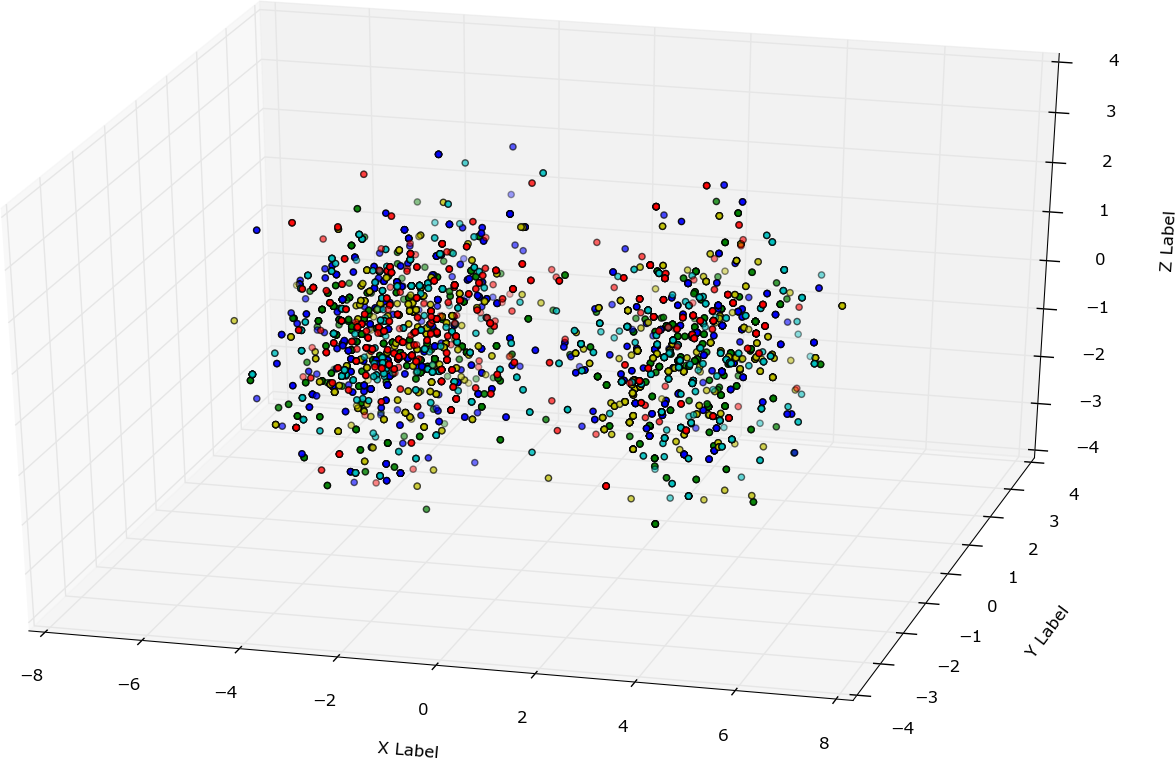
\includegraphics[width=0.69\textwidth]{figure_1}
  \vspace*{1mm}
  \subcaption{Optimal scaled acceptance probability with a good mixing between both modes.}
  \vspace*{3mm}
  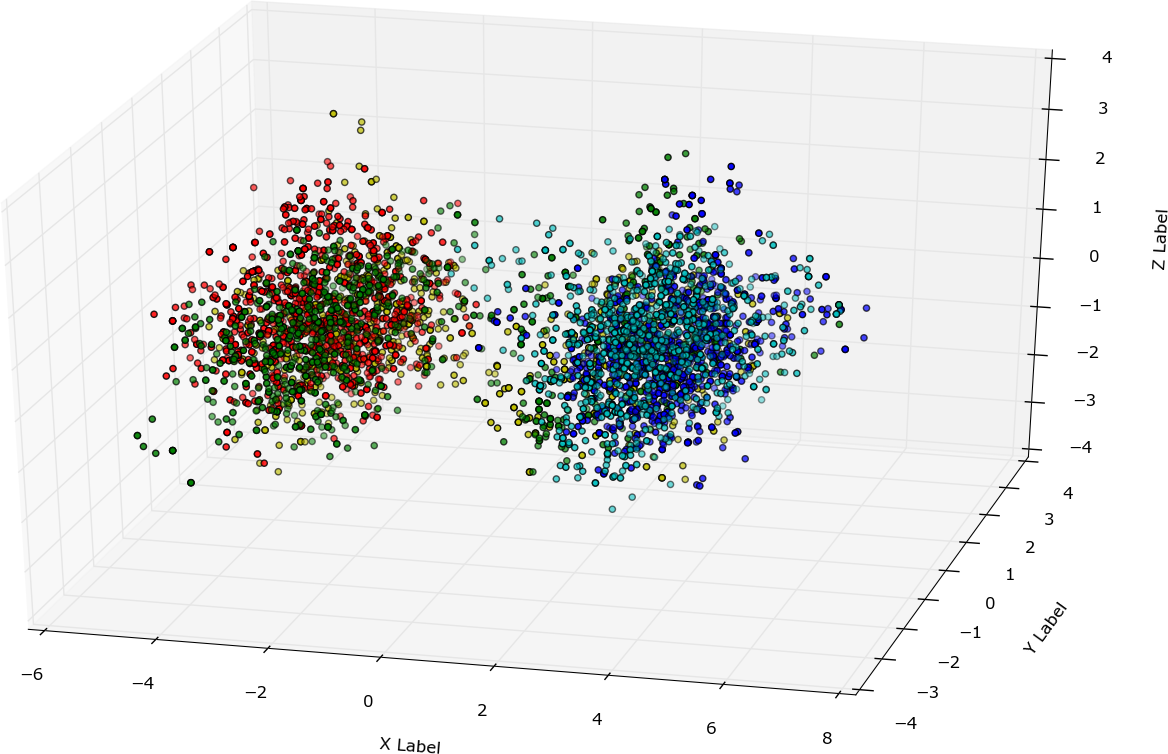
\includegraphics[width=0.69\textwidth]{figure_2}
  \vspace*{1mm}
  \subcaption{Too large acceptance probability with a bad mixing between both modes.}
  \vspace*{3mm}
  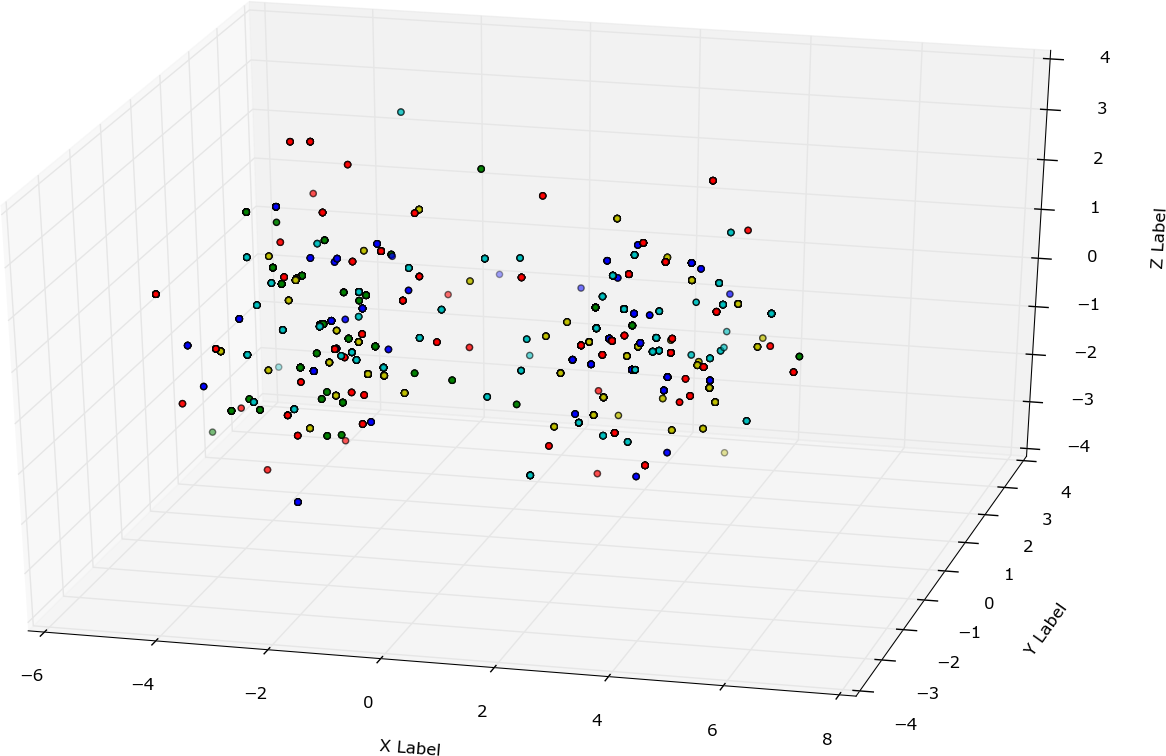
\includegraphics[width=0.69\textwidth]{figure_3}
  \vspace*{1mm}
  \subcaption{Too low acceptance probability.}
 \end{center}
  \caption{5000 samples produced by a RWM algorithm of a multimodal non-product target density. Every 1000 consecutive samples are labeled in the same colour.}
  \label{fig:3DscatterplotRWM}
\end{figure}

\subsection*{Own contributions}

My contributions to the present topic.
\begin{itemize}
 \item First point.
 \item Second point.
 \item Last point.
\end{itemize}


\subsection*{Outline}

A brief outline of the structure of this work.

Give an overview of present results of optimal scaling: Roberts and Rosental, Bedard, Breyer and Piccioni and Scarlatti, Mattingly and Pillai and Stuart and Thiery

\subsection*{Acknowledgements}

A list of persons, who deserve my acknowledgements: advisor, parents, friends.



 %introduction

\clearpage{\pagestyle{empty}\cleardoublepage} %begin next section at odd page and set remove header/footer

\section{The Metropolis-Hastings algorithm}
\label{sec:Metropolis-HastingsAlgo}

\subsection{The MCMC Principle}

\subsection{The Metropolis-Hastings algorithm}

\subsubsection{Convergence Properties}

\subsubsection{The Random Walk Metropolis-Hastings algorithm}

\subsubsection{The Metropolis adjusted Langevin algorithm}

\clearpage{\pagestyle{empty}\cleardoublepage} %begin next section at odd page and set remove header/footer

\section[Lorem ipsum]{Lorem ipsum - Testparagraph}

Lorem ipsum \autocite{Knuth:TeXbook} dolor sit amet, consetetur \autocite{pillai2012} sadipscing elitr, sed diam nonumy eirmod tempor invidunt ut labore et dolore magna aliquyam erat \autocite{roberts1997} , sed diam voluptua. At vero eos et accusam et justo duo dolores et ea rebum. Stet clita kasd gubergren, no sea takimata sanctus est Lorem ipsum dolor sit amet. Lorem ipsum dolor sit amet, consetetur sadipscing elitr, sed diam nonumy eirmod tempor invidunt ut labore et dolore magna aliquyam erat, sed diam voluptua. At vero eos et accusam et justo duo dolores et ea rebum. Stet clita kasd gubergren, no sea takimata sanctus est Lorem ipsum dolor sit amet. Lorem ipsum dolor sit amet, consetetur sadipscing elitr, sed diam nonumy eirmod tempor invidunt ut labore et dolore magna aliquyam erat, sed diam voluptua. At vero eos et accusam et justo duo dolores et ea rebum. Stet clita kasd gubergren, no sea takimata sanctus est Lorem ipsum dolor sit amet.   

Duis autem vel eum iriure dolor in hendrerit in vulputate velit esse molestie consequat, vel illum dolore eu feugiat nulla facilisis at vero eros et accumsan et iusto odio dignissim qui blandit praesent luptatum zzril delenit augue duis dolore te feugait nulla facilisi. Lorem ipsum dolor sit amet, consectetuer adipiscing elit, sed diam nonummy nibh euismod tincidunt ut laoreet dolore magna aliquam erat volutpat.   

\clearpage{\pagestyle{empty}\cleardoublepage} %begin next section at odd page and set remove header/footer

\appendix
\printbibliography

%\clearpage

\end{document}
